\documentclass[10pt,a4paper]{article}

\usepackage[margin=16mm,top=15mm,bottom=17mm]{geometry}
\usepackage[T1]{fontenc}
\usepackage[utf8]{inputenc}
\usepackage{lmodern}
\usepackage{amsmath}
\usepackage{microtype}
\usepackage{xcolor}
\usepackage{graphicx}
\usepackage{booktabs}
\usepackage{tabularx}
\usepackage{enumitem}
\usepackage{tcolorbox}
\usepackage{titlesec}
\usepackage{fancyhdr}
\usepackage[hidelinks]{hyperref}

\tcbuselibrary{skins,breakable}

% Palette
\definecolor{SkyPrimary}{HTML}{0369A1}
\definecolor{SkyLight}{HTML}{F0F9FF}
\definecolor{SkyBorder}{HTML}{BAE6FD}
\definecolor{EmeraldDark}{HTML}{047857}
\definecolor{EmeraldLight}{HTML}{ECFDF5}
\definecolor{AmberDark}{HTML}{B45309}
\definecolor{AmberLight}{HTML}{FFFBEB}
\definecolor{SlateDark}{HTML}{0F172A}
\definecolor{SlateMuted}{HTML}{475569}
\definecolor{SlateBg}{HTML}{F8FAFC}
\definecolor{BorderGray}{HTML}{CBD5E1}

% Section styling
\titleformat{\section}
  {\large\bfseries\color{SkyPrimary}}
  {}{0em}{}[\vspace{-4pt}\color{BorderGray}\rule{\linewidth}{0.8pt}]
\titlespacing*{\section}{0pt}{12pt}{6pt}

\titleformat{\subsection}
  {\normalsize\bfseries\color{SlateDark}}
  {}{0em}{}
\titlespacing*{\subsection}{0pt}{8pt}{3pt}

% Header & Footer
\pagestyle{fancy}
\fancyhf{}
\renewcommand{\headrulewidth}{0pt}
\fancyfoot[L]{\footnotesize\color{SlateMuted}\texttt{ID: 24B3972} \textbullet\ IntegerEase (Card P4--T1--L5--C4)}
\fancyfoot[R]{\footnotesize\color{SlateMuted}Page \thepage}

\setlist[itemize]{leftmargin=14pt, itemsep=2pt, topsep=3pt}
\setlist[enumerate]{leftmargin=16pt, itemsep=2pt, topsep=3pt}

\begin{document}

% Cover Banner
\begin{tcolorbox}[
  enhanced,
  colback=SkyPrimary,
  colframe=SkyPrimary,
  arc=6pt,
  boxrule=0pt,
  left=14pt, right=14pt, top=12pt, bottom=12pt
]
  {\footnotesize\bfseries\color{SkyBorder} ET 617--2026 \textbullet\ END-SEMESTER EXAMINATION REPORT}\\[4pt]
  {\LARGE\bfseries\color{white} IntegerEase: Calm 10-Minute Adaptive Integer Tutor}\\[5pt]
  {\small\color{SkyLight} Live App: \href{https://et617-24b3972.vercel.app}{\texttt{https://et617-24b3972.vercel.app}} \quad\textbullet\quad Repo: \href{https://github.com/rushilbhat01/ET617-Endsem-24B3972}{\texttt{github.com/rushilbhat01/ET617-Endsem-24B3972}}}
\end{tcolorbox}

\section*{Identity Card}
\begin{tabularx}{\linewidth}{@{}l X@{}}
\toprule
\textbf{Card Field} & \textbf{Specification} \\
\midrule
\textbf{Roll Number (ID)} & \texttt{24B3972} (displayed in footer of every screen and on \texttt{/about}) \\
\textbf{Exam Card} & \texttt{P4 -- T1 -- L5 -- C4} \\
\textbf{P4 -- Problem} & Adaptive tutor with automatic question generation (5 formats, explanation evaluation, 3-way decision rule) \\
\textbf{T1 -- Topic} & Integers: operations with negative numbers (Class 7) \\
\textbf{L5 -- Learner} & Learner repeating the topic after failing it once, high anxiety and low self-efficacy \\
\textbf{C4 -- Constraint} & 10-minute sessions: complete sequence fits in 10 minutes; stop and resume where left off \\
\textbf{Live URL} & \url{https://et617-24b3972.vercel.app} \\
\textbf{GitHub Repo} & \url{https://github.com/rushilbhat01/ET617-Endsem-24B3972} \\
\bottomrule
\end{tabularx}

\section*{D1. Educational Problem, Learning Outcomes \& Context of Use}
Class 7 learners repeating \emph{Integers: operations with negative numbers} often rely on memorized, fragile sign rules (e.g., ``two negatives make a negative'') rather than understanding direction on a number line or zero-pair cancellation. When applied inconsistently, these rules cause recurring sign errors---especially when subtracting negative numbers or comparing two negative values. Traditional practice platforms mark mistakes with punitive red indicators and generic hints, deepening math anxiety and lowering self-efficacy. An adaptive tutor that diagnoses \emph{why} a learner erred, switches to visual representations when needed, and structures practice into calm 10-minute sessions rebuilds both conceptual understanding and confidence.

\subsection*{Measurable Learning Outcomes}
By the end of a 10-minute session, the learner will be able to:
\begin{enumerate}
  \item \textbf{Compare \& Represent} positive and negative integers on a number line and with two-color counters to explain why $-2 > -5$.
  \item \textbf{Compute \& Predict} sums and differences of signed integers (including subtracting a negative integer, e.g., $-4 - (-2)$) using zero-pair or number-line reasoning.
  \item \textbf{Justify \& Debug} an integer operation in their own words, identifying and correcting common sign misconceptions.
\end{enumerate}
\textbf{Context of Use:} Evening study at home or an after-school study corner on a personal/shared smartphone or laptop, in calm 10-minute sessions with pause-and-resume.

\section*{D2. Learner Persona (Expanded from L5)}
\begin{tabularx}{\linewidth}{@{}l X@{}}
\toprule
\textbf{Dimension} & \textbf{Aarav Kulkarni (Class 7, Age 13)} \\
\midrule
\textbf{Prior Knowledge} & Fluent in whole-number arithmetic ($0$--$100$) and familiar with temperatures/elevators, but uncertain about negative ordering ($-8$ vs $-3$) and unfamiliar with zero pairs ($+1 + -1 = 0$). \\
\textbf{Misconception M1} & \textbf{Magnitude-Over-Sign / Direction Gap:} Treats $-8 > -3$ because $8 > 3$, moves the wrong direction on the number line, or gets the right magnitude with the wrong sign ($2 + (-5) = +3$). \\
\textbf{Misconception M2} & \textbf{Overgeneralized Sign Rule:} Believes ``two negatives always make a negative'' ($-4 - (-2) = -6$) or assumes subtraction always makes the result smaller. \\
\textbf{Device \& Language} & Mid-range Android phone or laptop; 10--15 minutes in the evening (\texttt{C4}); short, warm, conversational everyday English (\texttt{C3}). \\
\textbf{Motivation \& Affect} & High math anxiety and low self-efficacy (``I always mess up the minus signs''); responds well to non-punitive feedback, worked examples, peer debugging, and pre--post confidence tracking. \\
\bottomrule
\end{tabularx}

\section*{D3. Educational Content (Concept \& 5 Task Formats)}
Written in a conversational style (\texttt{P5}), the tutor pairs an \textbf{Interactive Number Line} ($-10$ to $+10$, keyboard and button accessible) and a \textbf{Two-Color Counter Board} ($+1$ yellow / $-1$ red with Zero-Pair cancellation) directly to \texttt{M1} and \texttt{M2}.

\begin{tabularx}{\linewidth}{@{}c l X l X@{}}
\toprule
\textbf{\#} & \textbf{Format} & \textbf{Task Prompt} & \textbf{Answer} & \textbf{Targeted Feedback (Correct / M1 / M2)} \\
\midrule
1 & \textbf{Number-Line} & Start at $-3$. Move to show $-3 + 5$. & $+2$ & \textbf{Correct:} Strategy praise + 5 right crosses $0$ to $+2$. \textbf{M1:} $+5$ moves RIGHT (warmer), not left. \\
2 & \textbf{Counter Board} & Build $2 + (-5)$, pair zero pairs, see what is left. & $-3$ & \textbf{Correct:} 2 zero pairs cancel; 3 red ($-1$) remain. \textbf{M1:} Check leftover color (red = negative). \\
3 & \textbf{Step-by-Step} & Solve $-4 - (-2)$ (Step 1: rewrite; Step 2: value). & $-4+2 \to -2$ & \textbf{Correct:} Removing 2 red tiles leaves $-2$. \textbf{M2:} Removing $-2$ debt goes UP to $-2$, not $-6$. \\
4 & \textbf{Error-Spotting} & Rohan wrote $-6 - (-3) = -9$. Spot the error! & Treated $-(-3)$ as $-3$ ($-3$) & \textbf{Correct:} Sharp eye spotting the sign trap. \textbf{M2:} Subtracting $-3$ removes 3 red tiles. \\
5 & \textbf{Written Explain} & Why does $3 - (-2)$ give $5$ instead of $1$? & Removing $-2$ adds $2$ & \textbf{AI-Evaluated:} Classifies into 5 classes and gives warm, specific feedback (with local fallback). \\
\bottomrule
\end{tabularx}

\section*{D4. Working Application \& Screen Map}
\textbf{Live URL:} \url{https://et617-24b3972.vercel.app} \quad\textbullet\quad \textbf{About:} \texttt{/about} \quad\textbullet\quad \textbf{Identity:} \texttt{ID: 24B3972} in every footer and on \texttt{/about}.
\begin{itemize}
  \item \textbf{State 1 --- Welcome / Resume (\texttt{WELCOME}):} Calm overview and \emph{Resume Where You Left Off} (\texttt{localStorage} persistence).
  \item \textbf{State 2 --- Randomized Diagnostic (\texttt{DIAGNOSTIC}, Part 1/4):} Dynamically generated negative comparison and subtraction-of-negative items plus an unbiased confidence check (no default selection).
  \item \textbf{State 3 --- Targeted Warm-up (\texttt{WARMUP}, Part 2/4):} Shows only the matched visual tool (Number Line or Counter Board) with a \emph{Try another way} toggle.
  \item \textbf{State 4 --- Adaptive Practice (\texttt{PRACTICE}, Part 3/4):} All 5 formats with zero repeats, \emph{$\leftarrow$ Review Warm-up}, \emph{See Similar Example}, \emph{Gentle Hint}, and \emph{Try Another Question}.
  \item \textbf{State 5 --- Adaptive Feedback (\texttt{ADAPTIVE\_FEEDBACK}):} \emph{Level Up}, interactive \emph{Visual Walkthrough} + \emph{Try This Question Again}, \emph{Quick 60-Sec Refresher}, or \emph{Quick Double-Check}.
  \item \textbf{State 6 --- Session Summary (\texttt{SUMMARY}, Part 4/4):} Active study time, tasks completed, and \textbf{Pre--Post Confidence Check}.
  \item \textbf{About \& Viva Controls (\texttt{/about}):} Identity card, repeatable Viva Demo Controls, and live local \texttt{eventLog} viewer.
\end{itemize}

\newpage
\section*{D5. Two Contrasting Learner Scenarios (Live App Screenshots)}

\subsection*{Scenario A --- Confident / Correct-Response Path (\texttt{HARDER\_QUESTION})}
Starting from 1 correct task, the learner selects $+2$ on the $-3 + 5$ Number Line with $0$ hints in $<60$\,s. The tutor triggers \textbf{Level Up $\cdot$ Challenge Task} and advances difficulty to Level 2.

\begin{figure}[h!]
  \centering
  \fbox{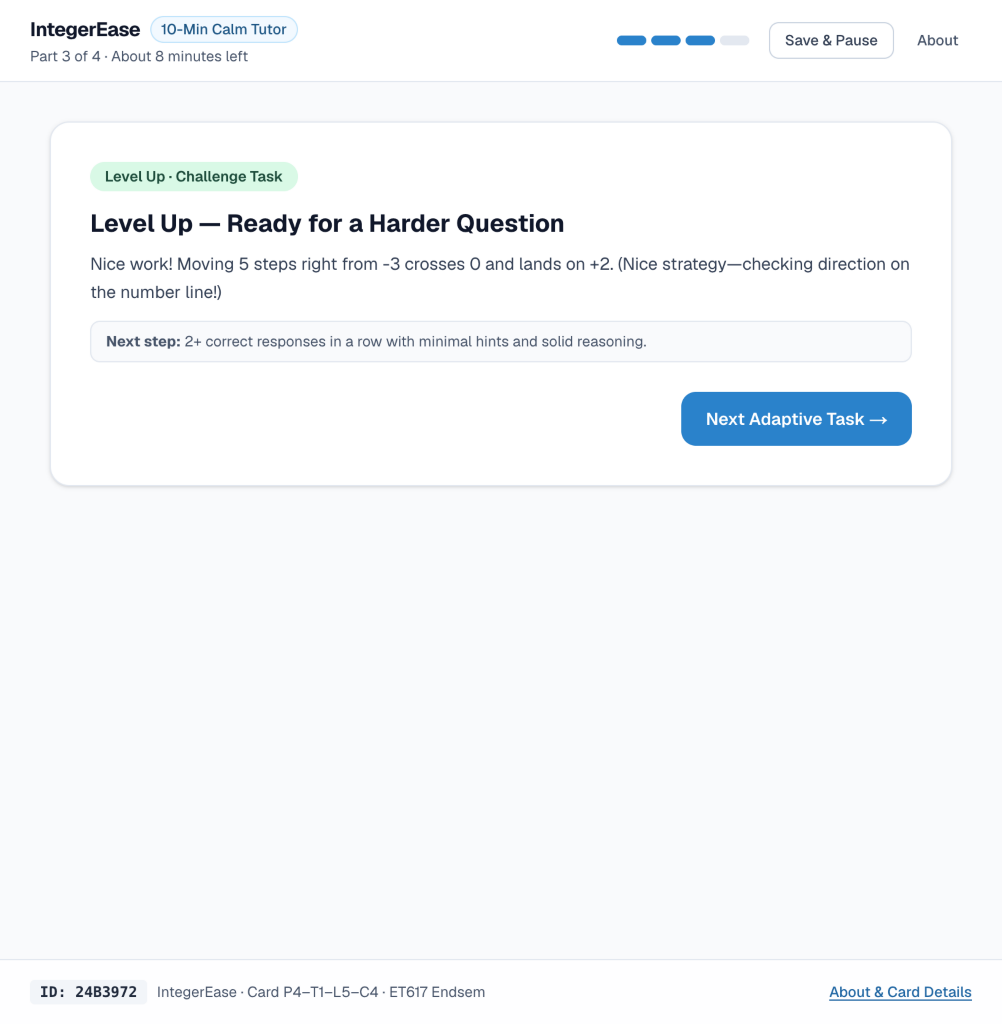
\includegraphics[width=0.92\linewidth,height=0.25\textheight,keepaspectratio]{screenshots/scenario-a-level-up.png}}
  \caption{Live Scenario A: Correct response on Number Line triggers \emph{Level Up $\cdot$ Challenge Task} (\texttt{ID: 24B3972} in footer).}
\end{figure}

\subsection*{Scenario B --- Misconception Path (\texttt{M2\_DOUBLE\_NEGATIVE})}
On $-4 - (-2)$, entering $-4 + 2$ and $-6$ once triggers \textbf{Visual Walkthrough} with the interactive Two-Color Counter Board; repeating $-6$ a second time escalates to \textbf{Quick 60-Sec Refresher}.

\begin{figure}[h!]
  \centering
  \fbox{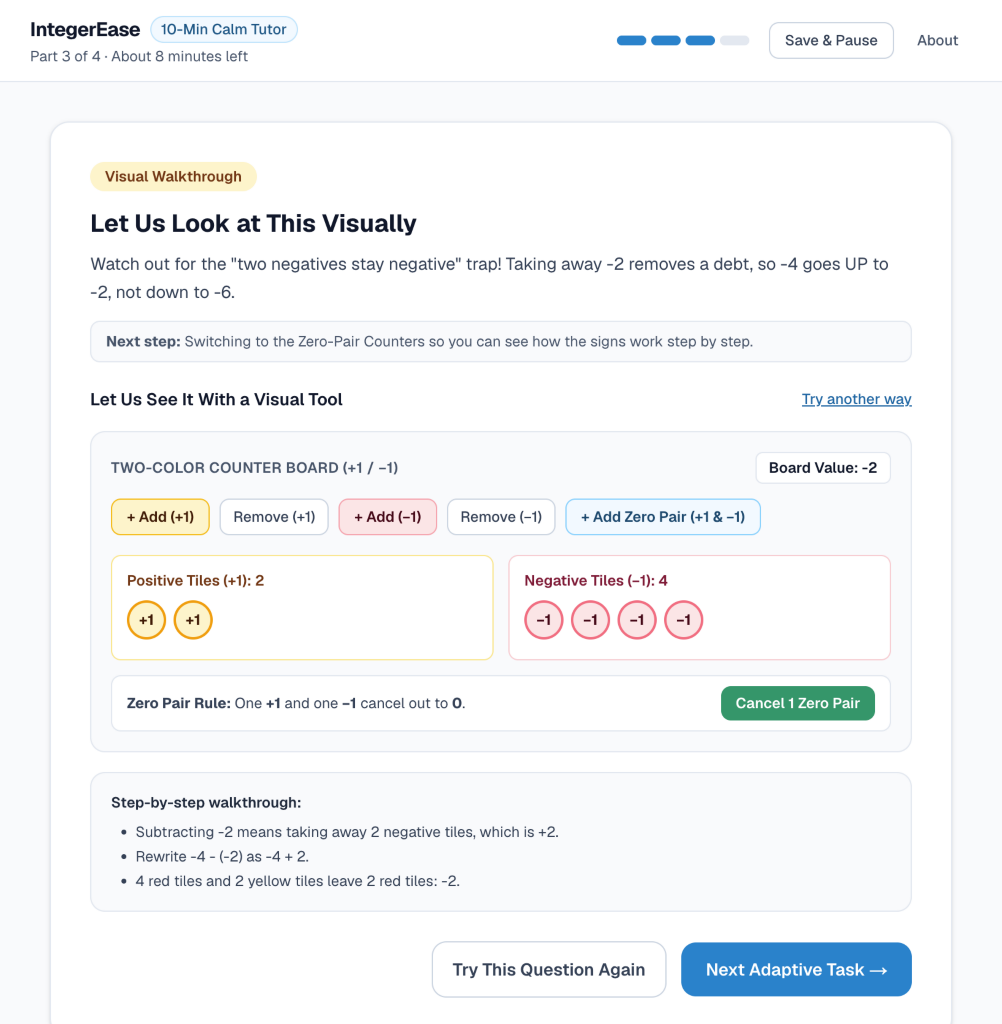
\includegraphics[width=0.92\linewidth,height=0.25\textheight,keepaspectratio]{screenshots/scenario-b-visual-walkthrough.png}}
  \caption{Live Scenario B (1st M2 occurrence): Switches to interactive Two-Color Counter Board + \emph{Try This Question Again}.}
\end{figure}

\begin{figure}[h!]
  \centering
  \fbox{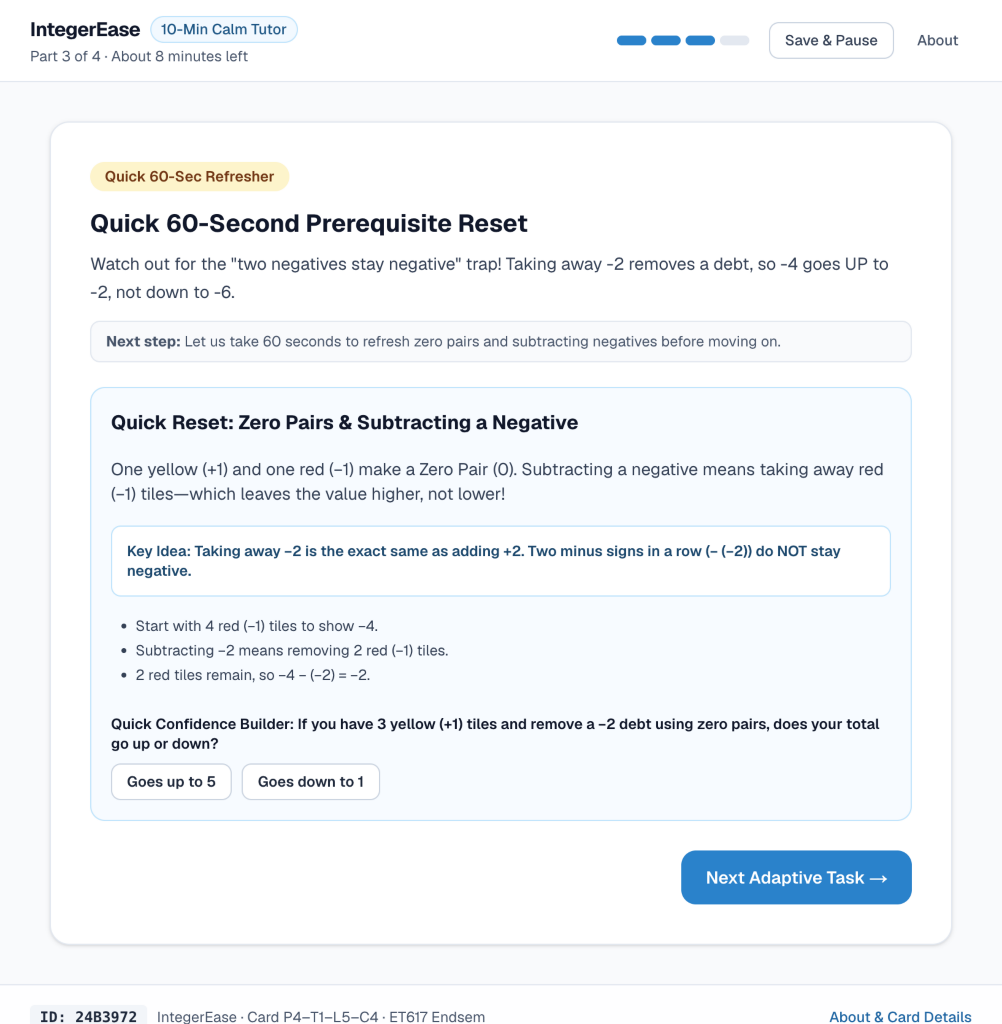
\includegraphics[width=0.92\linewidth,height=0.25\textheight,keepaspectratio]{screenshots/scenario-b-prereq-refresher.png}}
  \caption{Live Scenario B (2nd consecutive M2): Escalates to \emph{Quick 60-Sec Refresher} with \emph{Quick Confidence Builder}.}
\end{figure}

\newpage
\section*{D6. AI Functionality Specification (\texttt{/api/tutor})}
\begin{tabularx}{\linewidth}{@{}l >{\raggedright\arraybackslash}X >{\raggedright\arraybackslash}X >{\raggedright\arraybackslash}X@{}}
\toprule
\textbf{Feature} & \textbf{Model \& Input} & \textbf{Pre-Display Validation} & \textbf{Fallback} \\
\midrule
\textbf{Explanation Evaluator} & OpenAI \texttt{gpt-4o-mini} (JSON mode, temp 0.3) receives prompt, concept, model idea, and learner's text; classifies into 5 classes + feedback. & Checks \texttt{isCorrect} boolean, valid 5-class enum, valid \texttt{explanationQuality}, and non-empty feedback ($\le 400$ chars). & Local rule-based evaluator (\texttt{FALLBACK\_LOCAL}) using deterministic conceptual rules. \\
\textbf{Question Generator} & OpenAI \texttt{gpt-4o-mini} receives \texttt{targetDifficulty}, \texttt{focusMisconception}, \texttt{preferredFormat}, and \texttt{avoidPrompts}. & Schema check, integer range $[-10,10]$, negative integer check (\texttt{-\textbackslash d+}), duplicate prompt rejection, no answer leaks. & Non-duplicate curated item from \texttt{QUESTION\_BANK} (\texttt{FALLBACK\_BANK}). \\
\bottomrule
\end{tabularx}

\section*{D7. Pedagogical Rationale (Answering P4's Design Challenge)}
\begin{tcolorbox}[colback=SkyLight, colframe=SkyBorder, arc=4pt, boxrule=0.8pt, left=8pt, right=8pt, top=6pt, bottom=6pt]
  \textbf{P4 Decision Rule:} Combines \textbf{Profile} (randomized diagnostic), \textbf{Performance} (5-class diagnosis + Step 1 rewrite check), and \textbf{Interaction} (\texttt{hintsUsed}, worked examples viewed, \texttt{responseTimeMs}) to route to one of four evidence-based outcomes:
\end{tcolorbox}

\begin{tabularx}{\linewidth}{@{}X X@{}}
\begin{tcolorbox}[colback=EmeraldLight, colframe=EmeraldDark, arc=4pt, boxrule=0.6pt, left=8pt, right=8pt, top=6pt, bottom=6pt]
  \textbf{1. Harder Question (Level Up)}\\
  \small \texttt{isCorrect} + adequate explanation + $\text{hints} \le 1$ + $\text{time} \le 60$\,s + $\text{consecutiveCorrect} \ge 2$.
\end{tcolorbox}
&
\begin{tcolorbox}[colback=AmberLight, colframe=AmberDark, arc=4pt, boxrule=0.6pt, left=8pt, right=8pt, top=6pt, bottom=6pt]
  \textbf{2. Alternative Explanation (Walkthrough)}\\
  \small 1st clear \texttt{M1} or \texttt{M2}, or slow ($>60$\,s) unclear error. Pairs \texttt{M1} $\to$ Number Line; \texttt{M2} $\to$ Counter Board.
\end{tcolorbox}
\\
\begin{tcolorbox}[colback=SkyLight, colframe=SkyPrimary, arc=4pt, boxrule=0.6pt, left=8pt, right=8pt, top=6pt, bottom=6pt]
  \textbf{3. Prerequisite Instruction (Refresher)}\\
  \small \texttt{M1}/\texttt{M2} twice in a row, \textbf{2 consecutive scaffolded tasks} (hint/example), or diagnostic gap.
\end{tcolorbox}
&
\begin{tcolorbox}[colback=SlateBg, colframe=SlateMuted, arc=4pt, boxrule=0.6pt, left=8pt, right=8pt, top=6pt, bottom=6pt]
  \textbf{4. Gentle Retry (Double-Check)}\\
  \small \texttt{NON\_CONCEPTUAL\_SLIP} (off by 1 or Step 1 slip) or fast \texttt{UNCLASSIFIED}---never triggers remedial lessons.
\end{tcolorbox}
\end{tabularx}

\noindent\textbf{How L5 \& C4 Shaped Design:} No internal enum jargon on learner screens, unbiased confidence checks, worked-example toggles, calm skips, strategy praise, pre--post confidence tracking (\texttt{L5}), and 4-part pacing with \emph{Save \& Pause} + \texttt{localStorage} resume (\texttt{C4}).

\section*{D8. Evaluation Plan}
\begin{tabularx}{\linewidth}{@{}l X l X@{}}
\toprule
\textbf{D1 Outcome} & \textbf{Assessment / Rubric} & \textbf{Logged Signals} & \textbf{Success Criterion} \\
\midrule
1. Compare \& Represent & Diagnostic comparison + \texttt{NUMBER\_LINE} + \texttt{q-explain-2} & \texttt{DIAGNOSTIC\_COMPLETED}, \texttt{responseTimeMs} & $\ge 80\%$ resolve \texttt{M1} within 1--2 scaffolds. \\
2. Compute \& Predict & \texttt{COUNTER\_BOARD} + \texttt{STEP\_BY\_STEP} (Step 1 \& 2) & \texttt{RESPONSE\_SUBMITTED}, \texttt{HINT\_REQUESTED} & $\ge 75\%$ reach Level 2+ in $\le 10$ active mins. \\
3. Justify \& Debug & \texttt{ERROR\_SPOTTING} + \texttt{WRITTEN\_EXPLANATION} & \texttt{explanationQuality}, pre--post confidence & $\ge 70\%$ achieve \texttt{ADEQUATE} + positive shift. \\
\bottomrule
\end{tabularx}

\section*{AI-Use Log \& Reflection}
\textbf{AI Tools Used:} Antigravity coding assistant (architecture, Next.js/TypeScript implementation, live browser verification, and report generation) and OpenAI \texttt{gpt-4o-mini} (runtime explanation evaluation and question generation via \texttt{/api/tutor}). Complete chat logs are exported as \texttt{.txt} for Moodle.\\[4pt]
\textbf{Reflection:} Live testing caught four critical issues that initial AI generation missed: (1) internal enum names leaking into learner UI, (2) read-only walkthrough tools blocking exploration, (3) AI-generated prompts leaking answers ($5 + 3$) or omitting negative integers ($3 + 4$), and (4) Step 1 rewrite inputs needing explicit grading. Fixing each turned the prototype into a reliable, learner-centered tutor.

\end{document}
